\section{moMove$<$ EOT $>$ Class Template Reference}
\label{classmo_move}\index{moMove@{moMove}}
Definition of a move.  


{\tt \#include $<$moMove.h$>$}

Inheritance diagram for moMove$<$ EOT $>$::\begin{figure}[H]
\begin{center}
\leavevmode
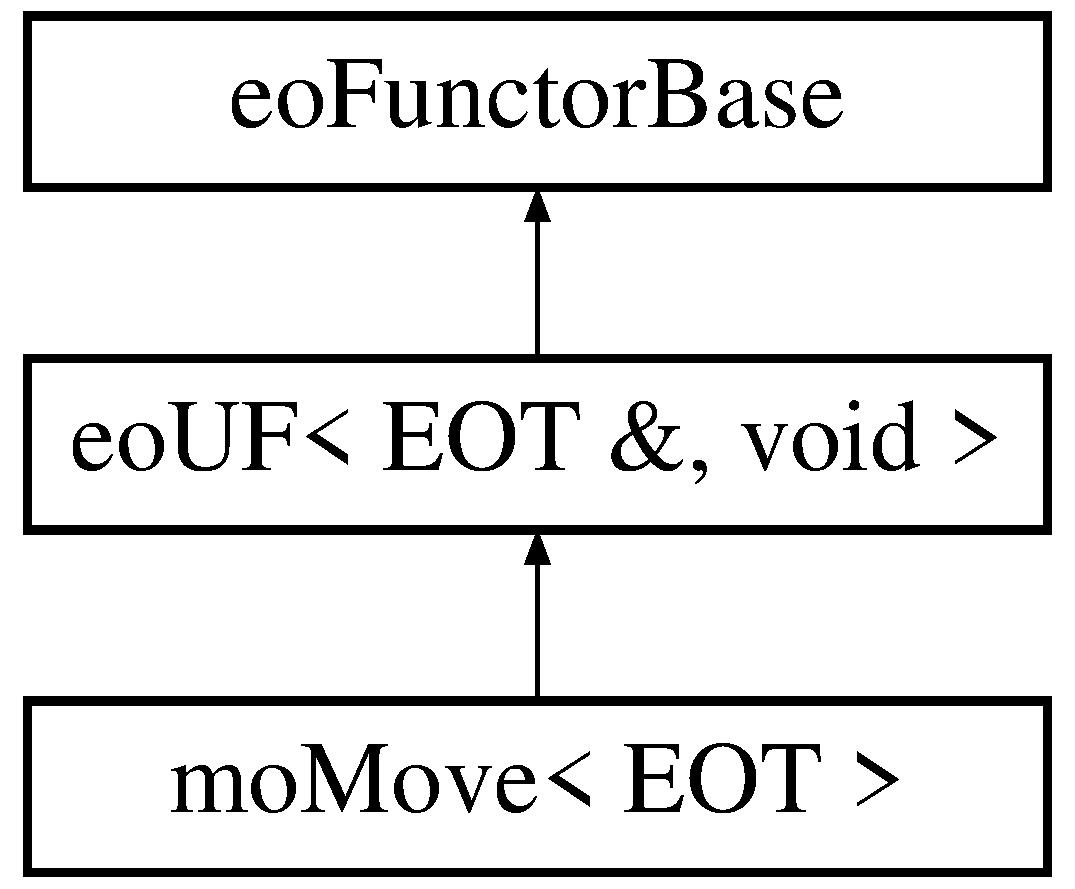
\includegraphics[height=3cm]{classmo_move}
\end{center}
\end{figure}
\subsection*{Public Types}
\begin{CompactItemize}
\item 
typedef EOT {\bf EOType}\label{classmo_move_7fb853a91ba1319530529e515380bbba}

\begin{CompactList}\small\item\em Alias for the type. \item\end{CompactList}\end{CompactItemize}


\subsection{Detailed Description}
\subsubsection*{template$<$class EOT$>$ class moMove$<$ EOT $>$}

Definition of a move. 

A move transforms a solution to another close solution. It describes how a solution can be modified to another one. 



Definition at line 23 of file moMove.h.

The documentation for this class was generated from the following file:\begin{CompactItemize}
\item 
moMove.h\end{CompactItemize}
